\chapter{Neutrino  experiments}
\label{c:expIntro}

%This chapter is aimed at putting the Baby MIND experiment into context of what has been done before, what experiments are under way and what experiments are planned.
\section{Neutrino detector experiments}
 
Since the discovery of the neutrino in 1956 by~\citeauthor{6Reines}~\cite{6Reines} a multitude of neutrino experiments have tried to measure the properties of the different neutrino flavours. Since the Homestake experiment many other experiments have been run to measure neutrino oscillations and the mass of the neutrinos. A detailed description of these experiments is outside of the scope of this thesis, in this section a description into the main types and milestones will be presented.

Neutrino experiments are split into three different categories based on the primary neutrino source. Each type features its own advantages and issues.
The detector types are:
\begin{itemize}
\item Atmospheric/Cosmic
\item Accelerator
\item Reactor
\end{itemize}
Each will be described briefly before examples are given.

\subsection{Atmospheric/Cosmic}

As mentioned in subsection \ref{subsection:Missing} neutrinos at different energy ranges are produced through nuclear interactions in stars. There are other cosmological phenomena which produce these neutrinos, and some searches are looking for signs of new physics in these signals. 

The Earth is constantly bombarded by cosmic-ray particles from space. When they hit the atmosphere, these high-energy protons interact with air molecules to produce showers of pions, which subsequently decay to muons and muon-neutrinos. This process is exactly similar to that used to produce neutrino beams from particle accelerators. Early observations of atmospheric neutrinos were contradictory, with some experiments observing approximately the expected ratio while others saw significantly fewer muon-neutrinos than expected, similar to the missing solar neutrinos, the Atmospheric Neutrino Anomaly. This was a measurement done by Super-Kamiokande and confirmed, together with the Homestake experiment, the existence of neutrino oscillations.

For these experiments either solar, or other cosmological sources are used to provide the neutrinos. The main advantages are that the energy can be very high, GeV to PeV range, and it is possible to use the earth to remove all background providing an extremely clean signal. However, it is impossible to control the source and difficult to get many events due to the low fluxes expected from astrophysical objects. In most cases the detectors are based on detecting Cerenkov light being emitted in a medium. Cerenkov light is emitted when a particle travels faster than the speed of light inside a medium. This creates a shock wave similar to the sonic boom that is visible in nuclear reactors as a bluish light.

\subsubsection{SNO}
The Sudbury Neutrino Observatory (SNO)~\cite{Fix6} was build to make a definite measurement of solar neutrinos following the measurements taken by the Homestake experiment~\cite{9Davis}. It utilized PMT (Photo Multiplier Tubes) to measure Cherenkov radiation produced by neutrino interactions in the detectors 1000 ton ultra-pure heavy water volume. The whole detector is placed 2 km underground to minimize background interactions. It expanded on looking for a specific energy range for cosmic rays, Boron decay, to becoming a generic neutrino detector meaning that other atmospheric and cosmic neutrinos became background events for measuring solar neutrinos.

\begin{figure}[h!]
\centering
\begin{subfigure}{.5\textwidth}
  \centering
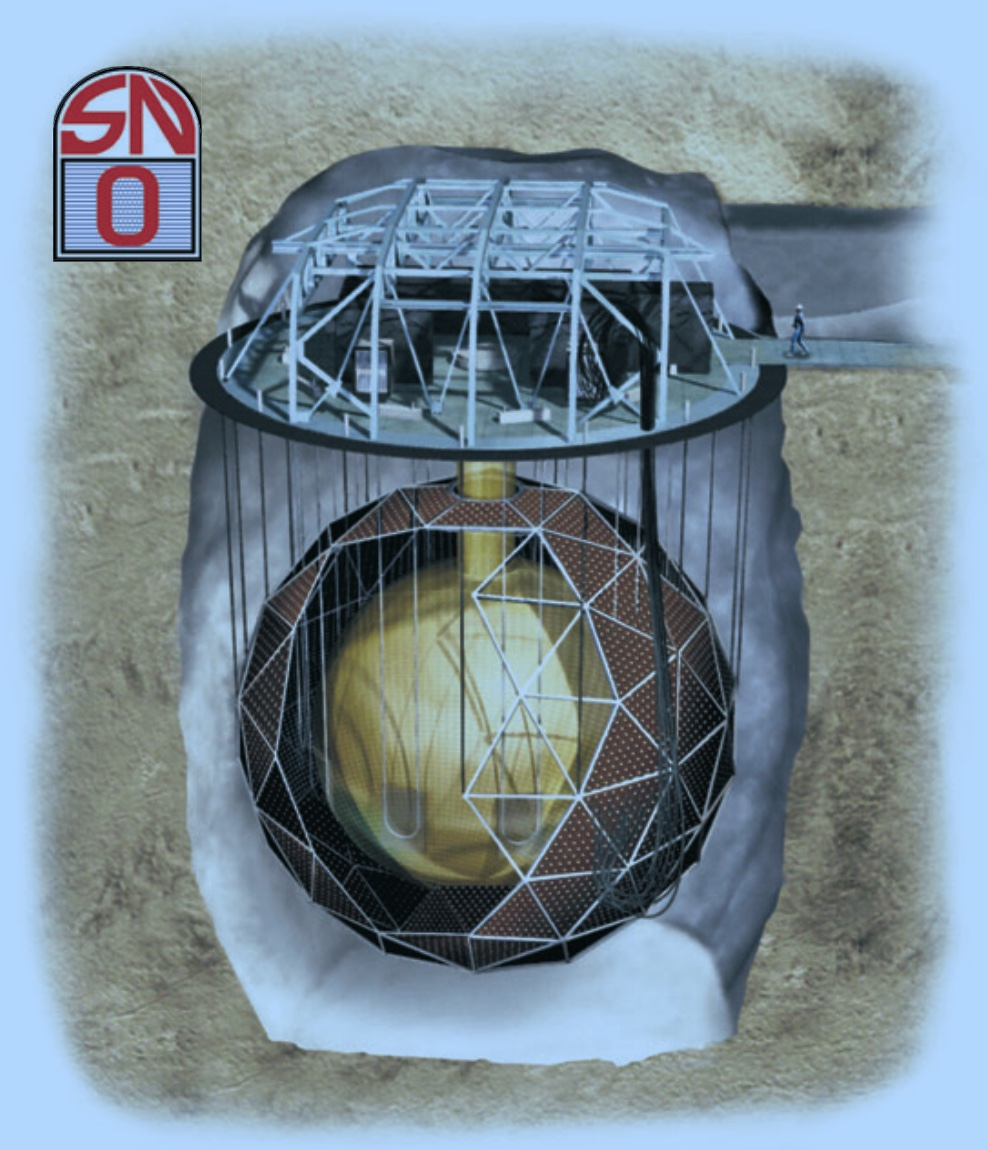
\includegraphics[width=0.7\textwidth]{figures/sno.jpeg}
\vspace{2mm}
  %\label{fig:sub1}
\end{subfigure}%
\begin{subfigure}{.5\textwidth}
  \centering
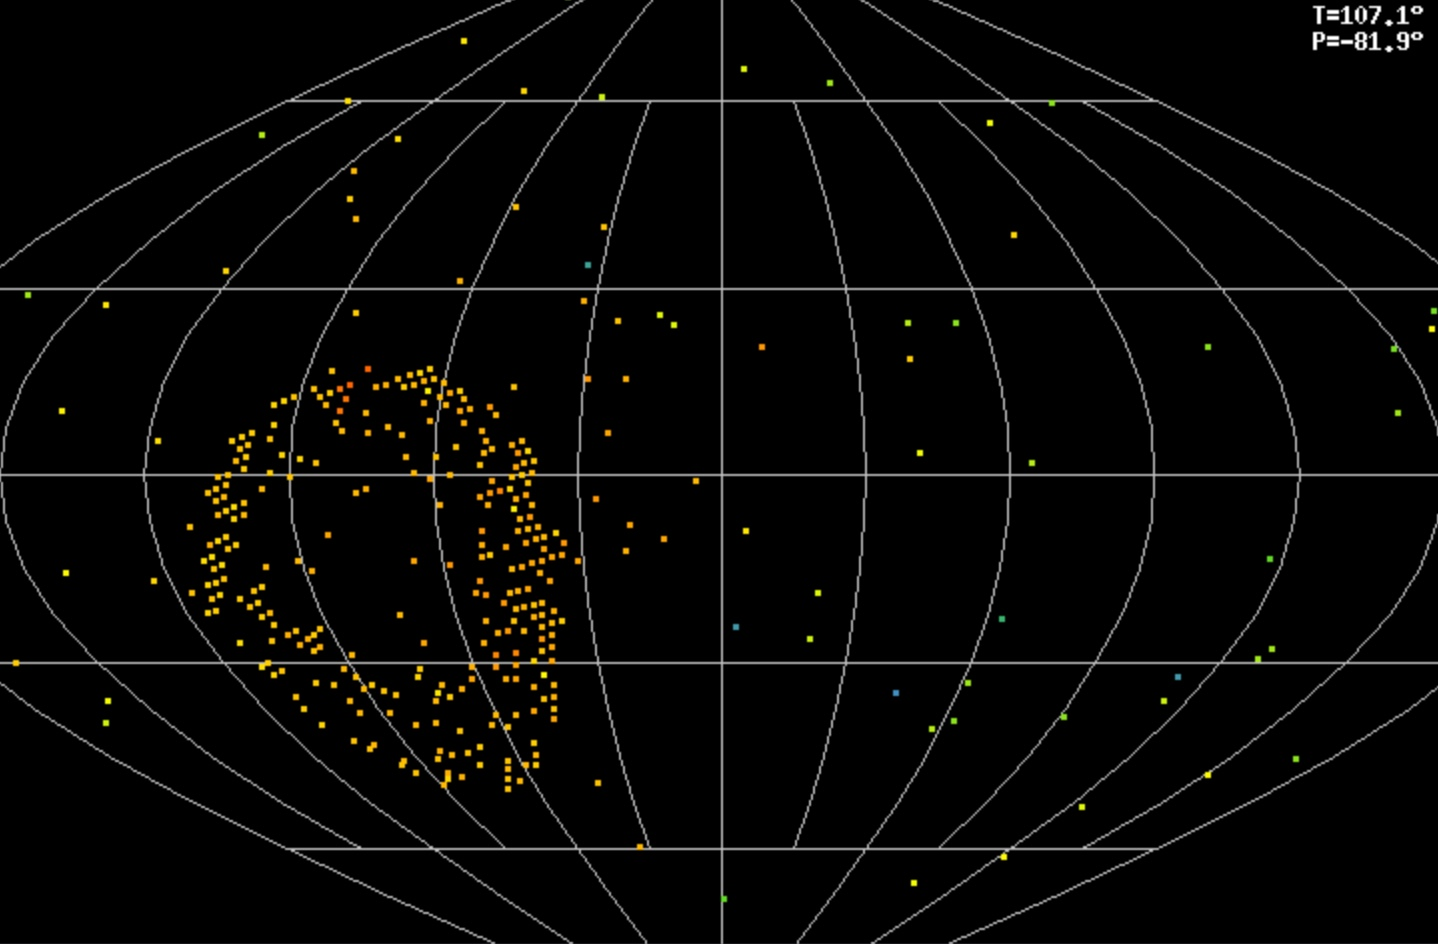
\includegraphics[width=\textwidth]{figures/SNOmuonEvent.jpeg}
\vspace{2mm}
  %\label{fig:sub2}
\end{subfigure}
\vspace{2mm}
\caption{Left) A schematic drawing of the SNO detector~\cite{Fix6}, Right) Cherenkov light recorded from a muon created by interaction of an atmospheric neutrino in the heavy water.}
\label{fig:SNO}
\end{figure}

The experiment is currently replacing the heavy water with liquid scintilator and renaming itself as SNO+~\cite{42SNO+}.

\subsubsection{Super-K}
Super-Kamiokande\cite{20SUPERK}, a water Cherenkov detector performed the first experimental observation that the neutrino has non-zero mass\cite{10Fukuda} and also managed to detect strong evidence of muon neutrino oscillation to tau neutrinos from the analysis of atmospheric neutrinos interacting in the water target. The Super-K is located 1 km underground and consists of a cylindrical stainless steel tank that holding 50 ktons of ultra-pure water. The detector is based on a similar design as the SNO detector. 

\begin{figure}[h!]
\centering
\begin{subfigure}{.5\textwidth}
  \centering
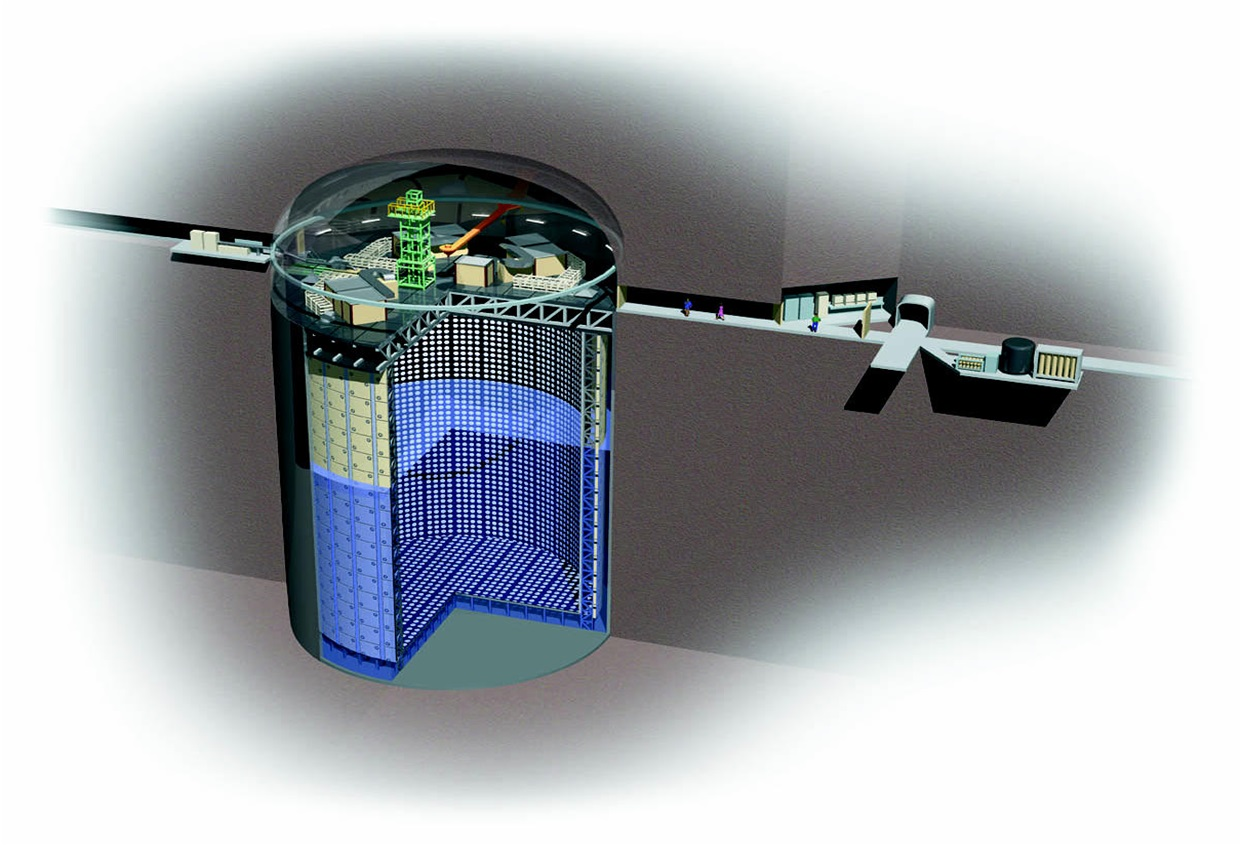
\includegraphics[width=\textwidth]{figures/SK3D.jpg}
\vspace{2mm}
  %\label{fig:sub1}
\end{subfigure}%
\begin{subfigure}{.5\textwidth}
  \centering
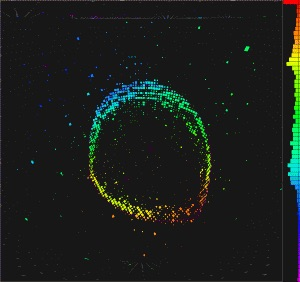
\includegraphics[width=0.7\textwidth]{figures/SuperKMuon-300x282.jpg}
\vspace{2mm}
  %\label{fig:sub2}
\end{subfigure}
\vspace{2mm}
\caption{Left) A schematic of the Super-K detector., Right) Event recorded in Super-K.}
\label{fig:SK}
\end{figure}
% http://t2k-experiment.org

\subsubsection{IceCube}
The IceCube observatory~\cite{43IceCube} also exploits the fact that particles produced in neutrino interactions emit Cherenkov photons. The low interaction probability of neutrinos require a large interaction volume. The South Pole offers a large interaction volume with very good optical qualities, using this is possible to instrument cubic kilometres of ice with a rather sparse spacing of detectors. The basic detection unit in IceCube is the digital optical module (DOM). The DOM contains, amount other things a PMT encapsulated in a glass pressure sphere to withstand the extreme pressure in the deep ice. In total 5160 DOMS are deployed, instrumenting a volume of one cubic kilometre of ice and allowing detection of astrophysical neutrinos in the energy range of TeV to PeV.

\begin{figure}
\centering
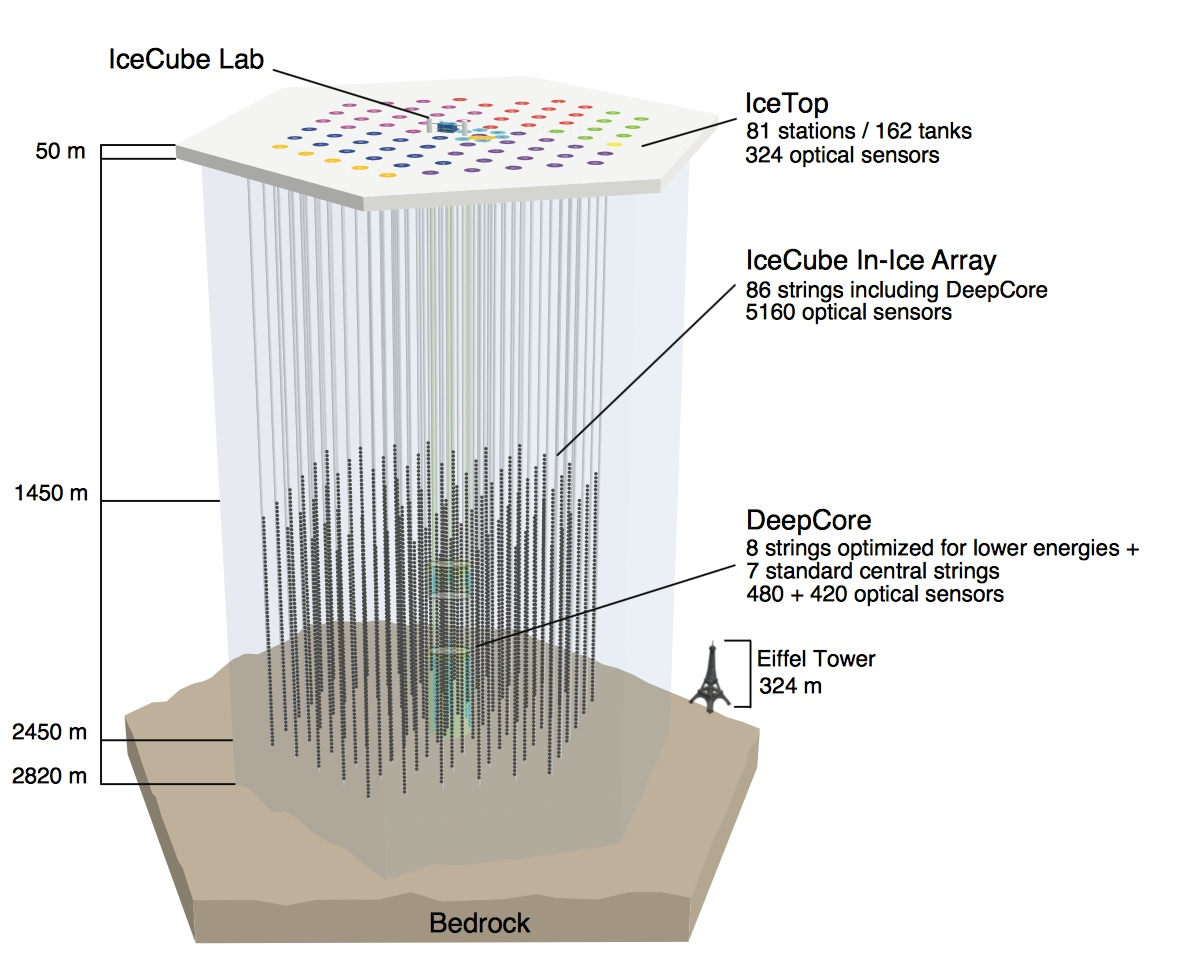
\includegraphics[width=.5\textwidth]{figures/IceCube.jpeg}
\caption{The IceCube Neutrino Observatory}
\end{figure}

\subsection{Accelerator}
Currently accelerator facilities can produce muon and electron neutrinos and anti neutrinos from accelerated protons. Protons are accelerated in a particle accelerator where the energy of the protons determines the energy of the neutrinos. The proton beam is then directed at a target where the protons interact with the target material, producing a large number of secondary pions (among other particles). Shaped magnetic fields, so called focusing horns, are used to select out pions of the preferred charge (positive for a neutrino beam, negative for an antineutrino beam) and focus them into a collimated beam. The beam is directed into a long decay volume, where the pions decay into muons and (anti)neutrinos. At the end of the decay volume there is a large mass of material which absorbs all the particles except the neutrinos. This provides a nearly pure beam of muon-neutrinos (or muon-antineutrinos if negatively charged pions are selected). There is some inevitable contamination with electron-neutrinos, mostly because the original pion beam also includes some kaons, which can decay to produce electron-neutrinos. To differentiate between these accelerator-based neutrino experiments, like reactor experiments, generally use a near detector as well as a far detector.

The advantage of accelerator neutrinos are that the energy range is well known and can be quite well tailored, the flux is huge compared to other methods. However the energy distribution will be quite wide because of the decay processes involved. It is also hard to produce a clean beam without background, muon neutrinos without electron neutrinos. However, for oscillation experiments this can be a good thing, see subsection \ref{subsec:nuFACT}.

\subsubsection{K2K / T2K}
After the success of Super-Kamiokande, the K2K-experiment\cite{22K2K} was created with the main difference of using a well understood muon neutrino beam pointing at the Super-Kamiokande detector at a distance of 250 km. It was the first neutrino oscillation measurement where both the source and detector were controlled, it observed the disappearance of muon neutrinos and found results that were consistent with Super-Kamiokande.

The next improvement came with the T2K-experiment\cite{21T2K}, which was also a long-baseline neutrino oscillation experiment with a more powerful beam from the JPARC facility at Tokai to Super-Kamiokande, at a distance of 295 km. The experiment wanted to improve the understanding of the neutrino oscillation parameters. T2K was able to successfully observe the appearance of muon to electron neutrino oscillations and find evidence that the third mixing angle $\theta_{13}$ is not zero. This is still an ongoing experiment. T2K  is comprised of a near detector, ND280 in Tokai, and a far site with the Super-K detector, see figure\ref{fig:T2K}.

\begin{figure}[h!]
\centering
  \centering
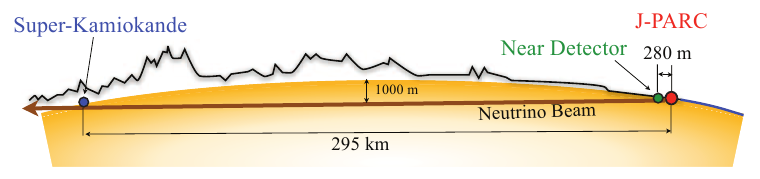
\includegraphics[width=\textwidth]{figures/T2KBeam.png}
\vspace{2mm}
\caption{A schematic view of the T2K experiment, including the near detector sight ND280 and Super-K.}
\label{fig:T2K}
\end{figure}

\begin{figure}[h!]
\centering
  \centering
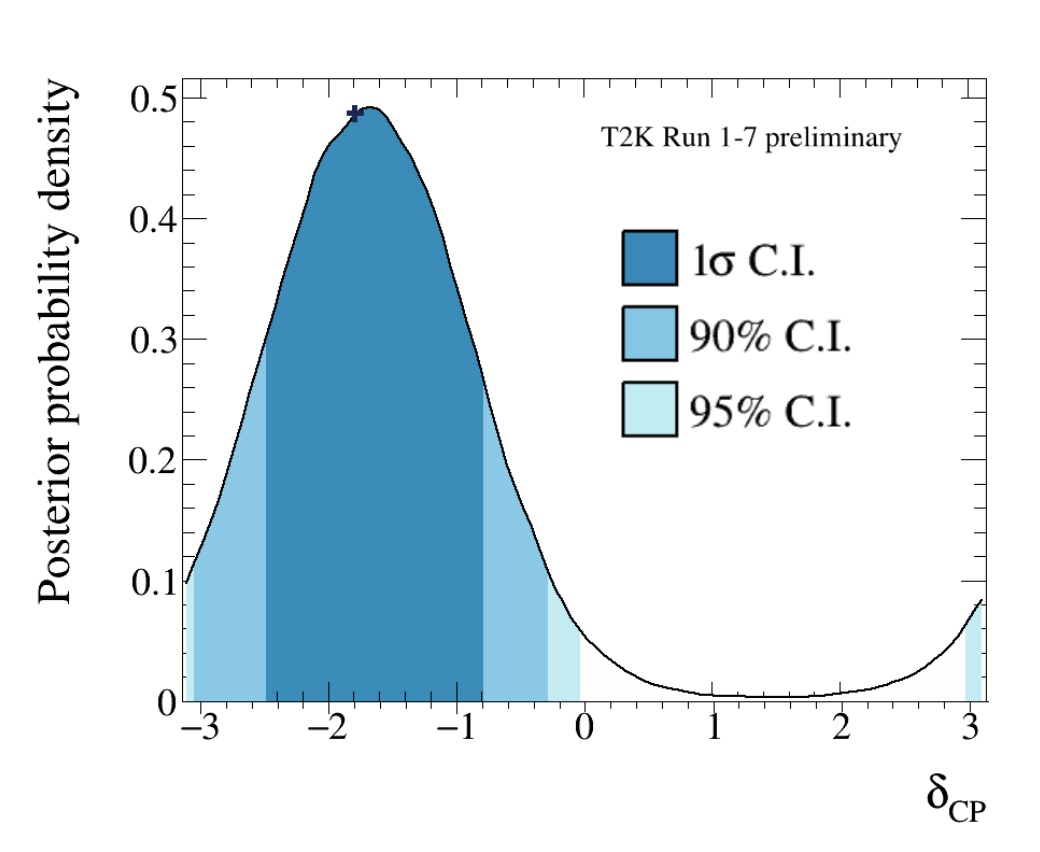
\includegraphics[width=0.7\textwidth]{figures/t2k1.jpeg}
\vspace{2mm}
\caption{Posterior probability density on $\delta$CP, where the cross represent the best-fit~\cite{T2Kfigures}.}
\label{fig:T2KCP}
\end{figure}

\begin{figure}[h!]
\centering
  \centering
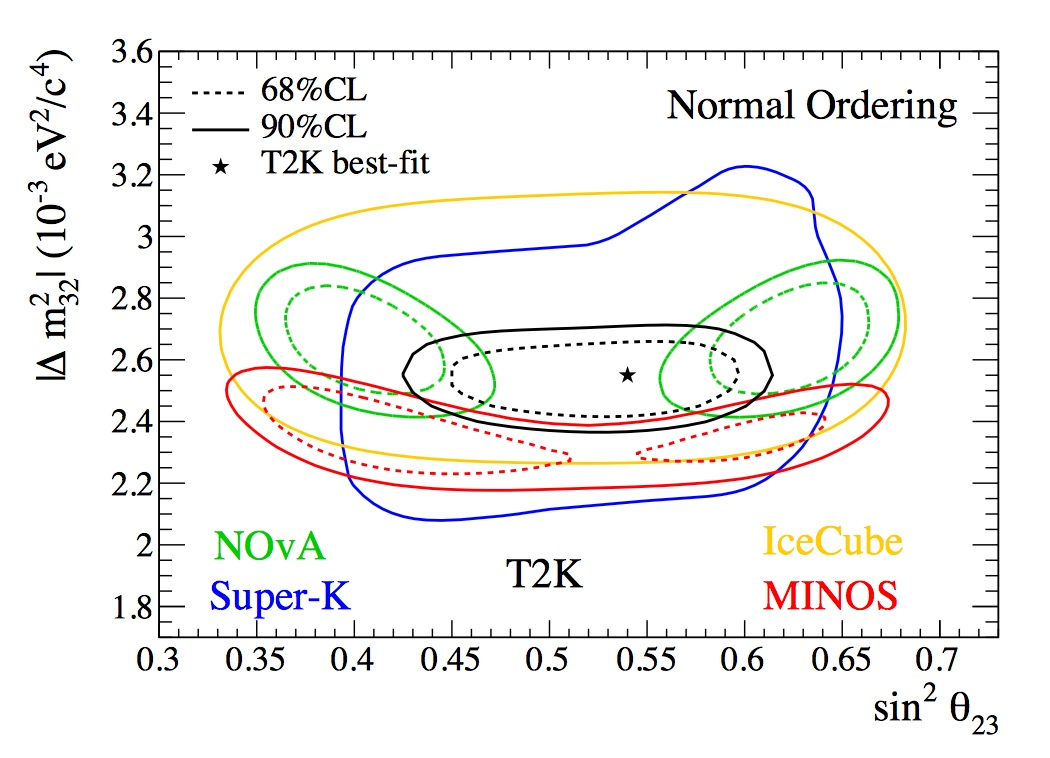
\includegraphics[width=0.7\textwidth]{figures/t2k2.jpeg}
\vspace{2mm}
\caption{The 90\% and 68\% confidence levels in the $\sin ^2 \theta_{23}-\Delta m^2_{32}$ space from T2K compared to other experiments, assuming normal ordering of neutrino masses~\cite{T2Kfigures}.}
\label{fig:T2K23}
\end{figure}

The main source of systematic error for T2K is caused by the difference of the target material and acceptance between the ND280 near detector (hydrocarbon) and the far detector water Cherenkov detector~\cite{T2Kpaper} motivating further studies and upgrades to the ND280 detector.

\subsubsection{CDHSW/NOMAD}
The European Organization for Nuclear Research, (CERN) has had accelerator neutrino experiments and some based around magnetised volumes to provide change identification of particles. 

The CERN Dortmund Heilelberg Saclay Warsaw (CDHSW)~\cite{40CDHSW} experiment was designed to study neutrino interactions in iron using the CERN SPS neutrino beam line. The experiment consisted of two similar detectors at different distances from the interaction vertex 130 m and 885 m~\cite{40CDHSW}.The detectors were built designed to combine the functions of a muon spectrometer and a hadron calorimeter. It consisted of 19 toroidal magnetised iron modules, with an average field of 1.65 T, separated from each other by wire drift chambers and had a mass of 1250 tons. In the end of the experiment a liquid hydrogen tank was placed in front of the experiment to study neutrino interactions in hydrogen.

%\textbf{RESULTS?}

The Neutrino Oscillation Magnetic Detector (NOMAD)~\cite{NOMADexp}, also using the CERN SPS neutrino beam line, searched for $\nu_\mu \rightarrow \nu_\tau$ oscillation by detecting $\tau$ appearance. Its goals were to measure the momenta of charged particles and identify and measure electron, photons and muons. By the detector design it was also possible to look for $\nu_\mu \rightarrow \nu_e$ oscillation. Compared to the modular design of CDHS, NOMAD had the drif chambers and other subdetectors contained inside a dipole magnet at 0.4 T.

%\textbf{RESULTS?}

\begin{figure}[h!]
\centering
  \centering
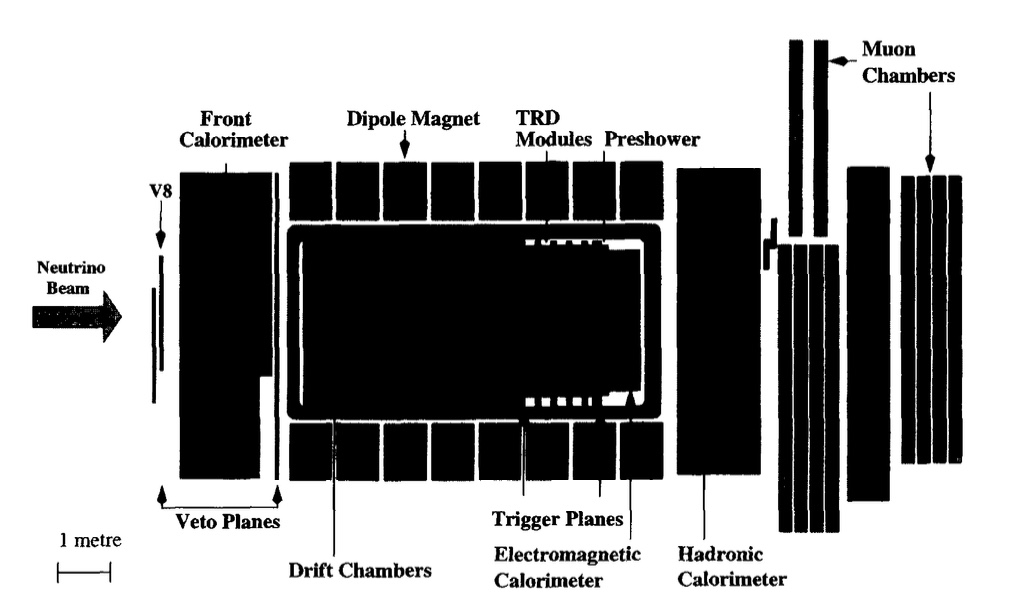
\includegraphics[width=\textwidth]{figures/NOMAD.jpeg}
\vspace{2mm}
\caption{A sideview of the NOMAD detector~\cite{NOMADexp}.}
\label{fig:NOMAD}
\end{figure}



\subsubsection{MINOS}
MINOS~\cite{MINOS} is also a muon neutrino disappearance experiment, consisting of one near and one far detector and using the NuMI~\cite{19NuMI} beam at Fermilab, to better understand the neutrino beam and showed results consistent with Super-Kamiokande and the K2K experiments. This is one of the first MIND (Magnetised Iron Neutrino Detector) types build along with CDHSW \cite{40CDHSW}. 

\if{0}
Mention NOMAD, CCFR/NuTeV

\subsubsection{NOvA}
After MINOS the next step using the NuMI~\cite{19NuMI} beam is the NOvA~\cite{18nova} experiment, which is also an electron neutrino appearance experiment and hopes to be able to determine the mass hierarchy of neutrinos.

\subsubsection{MINERvA}
The MINERvA (Main INjector ExpeRiment $\nu$-A)experiment \cite{39minerva} will also use the NuMI~\cite{19NuMI} beam to study neutrino-nucleus scattering to improve models of neutrino-nucleus scattering to reduce systematic uncertainties in results from oscillation experiments.

\subsubsection{MiniBooNE}
MiniBooNE\cite{41MiniBooNE} continued on what was started by MINOS but had the principle aim on improving neutrino mass measurements.

\fi

\subsection{Reactor}
Nuclear reactors are, compared to the other sources, very intense sources of low energy neutrinos. Through beta-decay channels both muon and electron neutrinos are produced with well known energy spectra and low background. Compared to the other neutrino sources the energy range is limited to be quite low. This means that oscillation experiments can be performed with a short baseline, use a small value for the momentum in \ref{eq:Problength} gives the same probability with a smaller length x.

\subsubsection{Double Chooz}
The Double Chooz experiment~\cite{45DoubleChooz} used anti-neutrinos produced two nuclear cores from a nuclear power station to improve the neutrino mixing angle $\theta_{13}$ as well as showed that these detectors can be used to ensure non-proliferation. The experiment consisted of two Cherenkov detectors at a distance of 280m and 1050m both consisted of PMTs inside a scintillating volume shielded from cosmic radiation. 

\begin{figure}[h!]
\centering
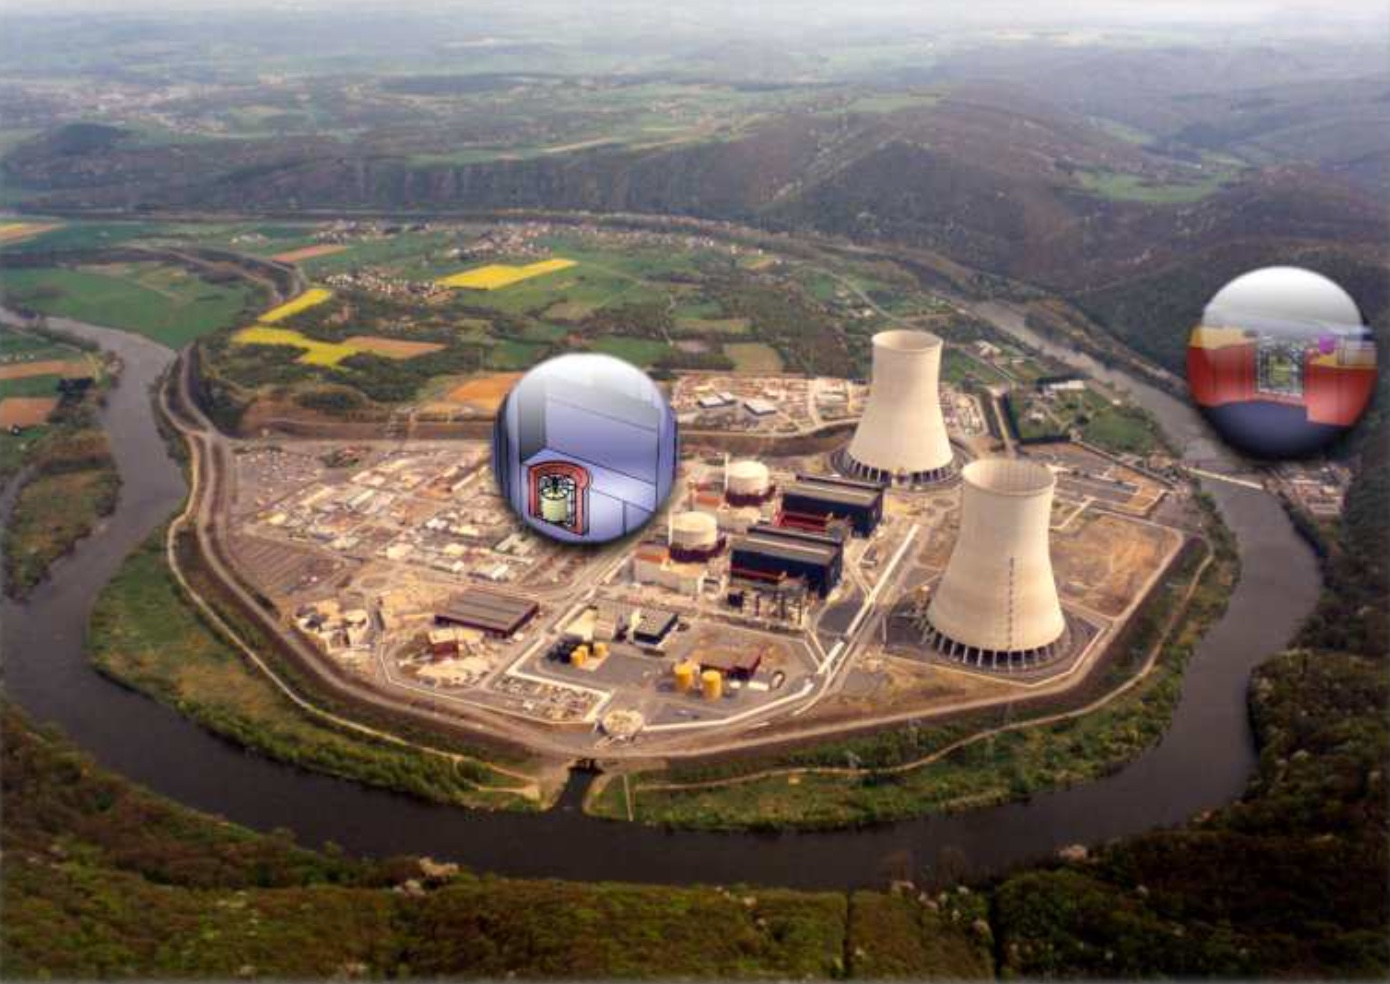
\includegraphics[width=0.6\textwidth]{figures/doubleChooz.jpeg}
\caption{Overview of the Double Chooz experimental site~\cite{45DoubleChooz}.}
\label{fig:dc}
\end{figure}

\subsubsection{Daya Bay}
The Daya Bay experiments~\cite{44DayaBay}, main goal is to improve the measurement of $\theta_{13}$It is improving results from Double Chooz by utilizing eight identical detectors placed at three locations around the Daya Bay area consisting of a total of 6 different nuclear cores. Each detector is a Cherenkov detector using PMTs.

\begin{figure}[h!]
\centering
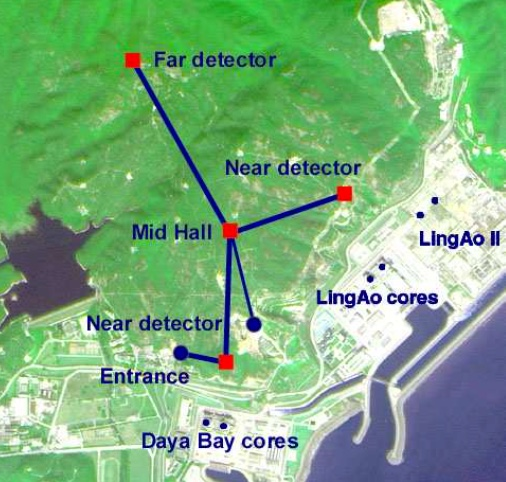
\includegraphics[width=0.4\textwidth]{figures/DayaBay.jpeg}
\caption{Layout of the Daya Bay experiment.~\cite{44DayaBay}.}
\label{fig:DB}
\end{figure}
\if{0]
\subsubsection{KamLAND}
KamLAND, the Kamioka Liquide scintilator Anti-Neutrino Detector, was build in 2002 and helped investigate if there were any neutrino oscillations by looking at anti electron neutrinos emitted from distant reactors~\cite{46KamLAND}.
\fi
%\subsection{Summary of important discoveries}
%\textbf{Table, different mass and so on.}
%\subsection{Current limits}

\section{Future neutrino oscillation experiments}
%\subsection{KATRIN}

\subsection{Hyper-K}
The Hyper-Kamiokande Experiment\cite{24HyperK}  builds on the T2K-experiment\cite{21T2K} by improving the neutrino beam at JPARC, and expanding the water Cherenkov detector by a factor of 10 to a fiducial volume of 500 ktons, which aims to improve the sensitivity for $\delta_{cp}$.

\if{0}
\subsection{DUNE}
LBNF/DUNE\cite{23DUNE} is a new experiment aiming at looking at the full range of $\delta_{cp}$ with greater sensitivity than before by improving on the MINOS~\cite{MINOS} experiment, and performing an electron neutrino appearance measurement with a high-powered neutrino beam from Fermilab and a 40 kton liquid argon detector at a distance of 1300 km, in the Homestake mine in South Dakota.
\fi
\subsection{nuStorm experiment/Neutrino factory}\label{subsec:nuFACT}
The Neutrino Factory (NuFACT) is a novel concept for a neutrino accelerator which will produce a high intensity (1000 higher than previously) and high energy beam (up to 20-50 GeV). Compared to other previous experiments it will produce a two flavour, electron and muon, neutrino beam through a muon decay ring. The neutrino factory has the capacity to improve the precision of neutrino oscillation measurements, since the neutrino beam from the decay of muons can be determined with high accuracy. The beam produces one bunch of $\mu^+$ and one bunch of $\mu^-$, so the facility can make measurements of $\nu_{\mu}$ and $\bar{\nu_{e}}$ and $\bar{\nu_{\mu}}$ and $\nu_{e}$ simultaneously. Using this $\delta_{cp}$ can be decisively explored, with an expected accuracy of $\Delta \delta_{CP}\sim 5^\circ$~\cite{25NUfact}. NuFACT is also significantly better that alternative facilities at measuring the value if $\theta_{13}$ is small. A schematic of the facility is shown in figure \ref{fig:nuFact} showing the full accelerator chain. The full chain, starts by producing muons and pions from a proton beam on target. The particles are selected based on charge in a magnetic horn after which the pions decay into muons in a transport line before the beam being collating to form a pure muon beam. The muon beam is then cooled to focus the beam before further accelerating the muon beam to its final energy and introducing it into the decay ring. After $\approx 70$ turns of the circuit the muons decay through the following modes with the branching ratio:

\begin{align}
\mu^- &\rightarrow e^- + \bar{\nu_e} + \nu_\mu, \approx 100\% \\
\mu^- &\rightarrow e^- + \bar{\nu_e} + \nu_\mu + \gamma, <1\% \\
\mu^- &\rightarrow e^- + \bar{\nu_e} + \nu_\mu + e^+ + e^-, <1\%
\end{align}

From the branching ratio the energy spectrum and competition of the neutrino beam is well known, The beam is also produced as a pure beam since they are two neutrino flavours at the same time but with different flavours. It is important to know that a muon beam will only produce muon neutrinos and anti-electron neutrinos. Thus any electron neutrinos or anti-muon neutrinos discovered must have been produced through oscillation. Currently there are proposals for NuFACT to be constructed at CERN~\cite{25NUfact}, ESS~\cite{ESS} and FERMILAB~\cite{NuFACTfermi}, where it is also seen as a step toward a full muon collider experiment.
%Neutrino factory, explain it. MIND detector for nufact.  MIND needed for charge id, wrong sign muons produced from mu neutrino and anti electron neutrino in accelerator, anti electron to anto muon oscillation. Nufact known 0 anti nu mu in generation, only in oscillation. Prob is 0 for nufact for wrong sign at near detector/source.

\begin{figure}[h!]
\centering
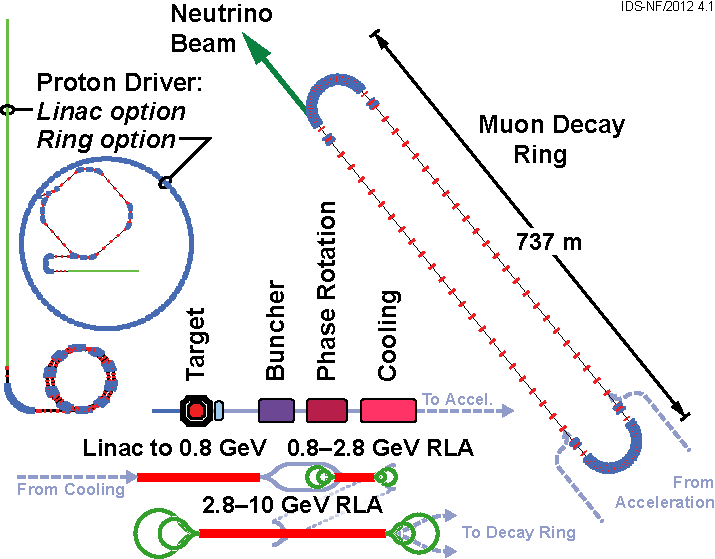
\includegraphics[width=0.9\textwidth]{figures/131112-IDS-NF.pdf}
\caption{Schematic diagram of the Neutrino Factory~\cite{Fix7}.}
\label{fig:nuFact}
\end{figure}

\begin{figure}[h!]
\centering
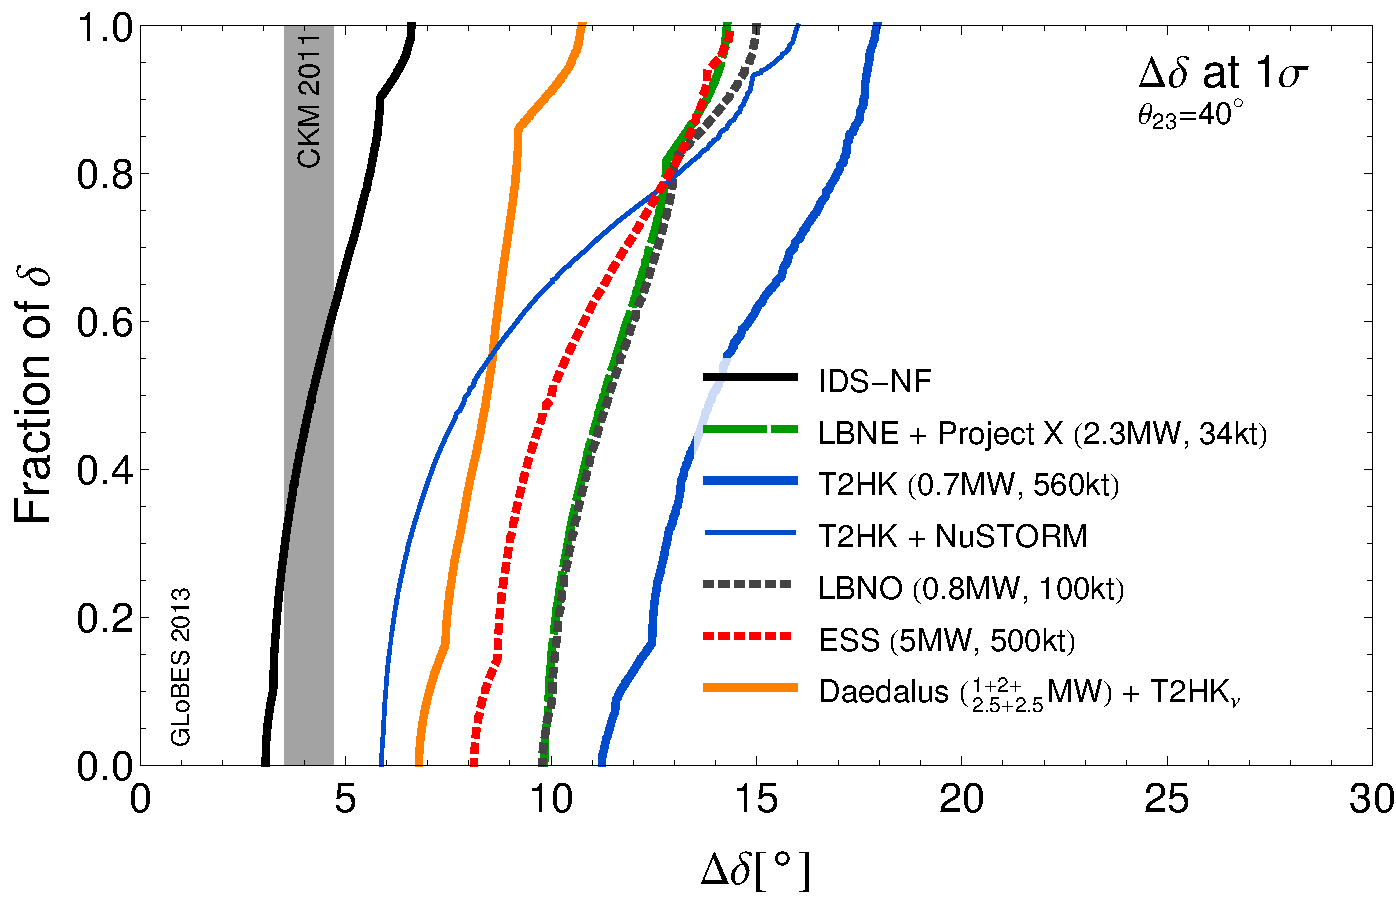
\includegraphics[width=0.9\textwidth]{figures/rdr-cp-precision-comparison-131216.pdf}
\caption{Expected precision for a measurement of the $\delta_{cp}$ at a Neutrino Factory compared to alternate neutrino oscillation facilities~\cite{Fix7}.}
\label{fig:nuFactExp}
\end{figure}

The Neutrino Factory is an complex and expensive facility which requires new technology to be realised. To overcome this a staged approach has been suggested, where each stage would be delivering physics~\cite{Fix7}. The first state in this plan is named nuSTORM (Neutrinos from Stored Muons) with a schematic shown in figure~\ref{fig:nuStorm}. The nuSTORM beam is designed to produce 3.8 GeV/c muons which are injected into a muon storage ring. Compared to the full neutrino factory nuSTORM is expected to have some pions and kaons in the final beam producing both neutrinos and anti-neutrinos for both muon and anti-muon modes and thus a near detector is required to measure the flux of both. 

\begin{figure}[h!]
\centering
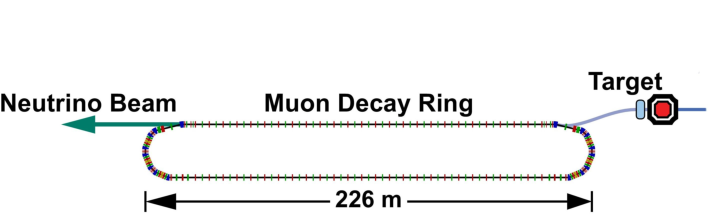
\includegraphics[width=\textwidth]{figures/nuSTORM_schematic.pdf}
\caption{A schematic of a nuSTORM facility~\cite{Fix7}.}
\label{fig:nuStorm}
\end{figure}

For the both NuFACT and nuSTORM the detector type proposed will be a MIND type, similar to the ones used in CDHSW and MINOS~\cite{NuFACTIDS}.



\section{Magnetized Iron Neutrino Detectors}\label{subsec:MINDdetector}
Magnetized Iron Neutrino Detectors (MINDs) have been operated in several experiments such as CDHSW~\cite{40CDHSW} and MINOS~\cite{MINOS}. This type of detector, with magnetized steel plates and scintillation plates, is well suited to provide large mass for neutrino experiments and is able to provide momentum measurements by using range and curvature calculations as well as providing charge identification. A MIND type detector has been selected as the baseline detector for a neutrino factory~\cite{ISS, 27Bross}, since it is the cheapest and most effective way of producing a large magnetized volume. This has provided the motivation for creating a prototype detector to perform a number of studies.

Since water Cherenkov and liquid argon detectors have been established or actively studied for future very large scale neutrino oscillation experiments, a MIND type detector is not foreseen to be used as the main interaction medium for any planned upcoming experiments.. A MIND type detector can however be used to provide charge identification of muons if positioned downstream of any neutrino target which is not magnetized.

%==============================================================================
